\documentclass[12pt]{article}

\usepackage[T1]{fontenc}
\usepackage[polish]{babel}
\usepackage[utf8]{inputenc}
\usepackage{lmodern}
\selectlanguage{polish}

\usepackage{graphicx}
\usepackage{tabularx, booktabs}
\usepackage{fancyhdr} 
\usepackage{geometry}
\usepackage{hyperref}
\usepackage{listings}
\usepackage{float} 
\usepackage{subfigure}

\usepackage{a4wide}

\geometry{left=15mm,right=25mm,%
bindingoffset=10mm, top=20mm, bottom=20mm}
 


\renewcommand{\maketitle}{
\begin{titlepage}
\begin{table}[t]
\centering
\begin{tabular}[t]{lcr}
 
\includegraphics[width=70pt,height=70pt]{PW} & POLITECHNIKA WARSZAWSKA & 
\includegraphics[width=70pt,height=70pt]{MiNI}\\
& WYDZIAŁ MATEMATYKI & \\
& I NAUK INFORMACYJNYCH &
\end{tabular}
\end{table}
\vspace*{3cm}
  \begin{center}
    \LARGE
    \textbf {MSI2 - Raport}\\
   \vspace*{2 cm}
\begin{table}[!htp]
\begin{tabular}{p{4cm}p{9cm}}
\textit{Przedmiot:} &\textbf {Metody sztucznej inteligencji 2} \\
\\
\textit{Projekt:} &\textbf {Agent do grania w gry Atari przy użyciu uczenia wzmocnionego (reinforcement learning)} \\
\\
\textit{Autorzy:} &\textbf {Michał~Kołodziej \newline Nikodem~Wiśniewski} \\
\\
\end{tabular}
\end{table}

\vspace{5 cm}
  \center{\small Warszawa, dnia \today}
\end{center}
\end{titlepage}
}

\begin{document}
\maketitle


\section{Opis projektu}
Zadaniem tego projektu jest stworzenie agenta komputerowego grającego w gry z Atari 2600 \cite{atari}. Agent jest trenowany za pomocą uczenia przez wzmacnianie (reinforcement learning) poprzez samoczynne granie w wybrane gry. Podczas uczenia agent miał styczność z wieloma grami z konsoli Atari takimi jak: Breakout, Pong, Atlantis czy Krull.

\section{Metodyka}

Do uczenia agenta zostało użyte środowisko OpenAI Gym \cite{gym} z rozszerzeniem o symulator gier Atari. Środowisko to udostępnia API do wyświetlania ekranu emulatora, wykonywania kolejnych akcji w emulatorze, resetowania stanu gry, pobierania informacji z emulatora takich jak: zrzut ekranu emulatora, informacja o nagrodzie po wykonaniu akcji, informacja o zakończeniu się rozgrywki. Podczas uczenia agent ma przedstawione jako stan 4 ostatnie klatki z gry, na podstawie których wybiera akcje do wykonania w danym stanie. Dzięki temu ma on nie tylko podgląd obecnego zrzutu ekranu, ale również widzi dynamiczne zmiany zachodzące w grze. Z emulatora pobierane są zrzuty w rozmiarze $160\times210$ pikseli w przestrzeni barw RGB. W celu ograniczenia ilości przetwarzanych danych rozmiar każdej klatki jest skalowany i obcinany do $84\times84$ pikseli, a 3 kanały koloru są rzutowane na jeden kanał w 256 wymiarowej skali szarości.
\\\

\begin{figure}[H]%
\centering
\subfigure[Klatka z emulatora]{%
\label{fig:first}%
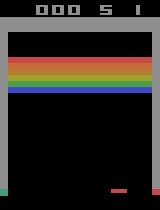
\includegraphics[scale=0.5]{1_raw.jpg}}%
\qquad
\subfigure[Klatka w skali szarości]{%
\label{fig:second}%
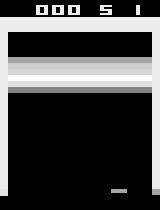
\includegraphics[scale=0.5]{2_gray.jpg}}%
\qquad
\subfigure[Klatka przeskalowana]{%
\label{fig:third}%
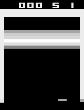
\includegraphics[scale=0.5]{3_resized.jpg}}%
\qquad
\subfigure[Klatka obcięta]{%
\label{fig:fourth}%

\includegraphics[scale=0.5]{4_cropped.jpg}}%
\caption{Kolejne kroki przetwarzania obrazu wejściowego}
\end{figure}



\subsection{Nagrody}

Na poączątku należy zdefiniować pojęcie nagrody w kontekście nauczania ze wzmocnieniem. Agent za każdą akcję dostaję nagrodę i dąży do maksymalizacji nagród w trakcie jednej gry. Aby uniezależnić agenta od konkretnych gier (każda gra ma swoją skalę punktacji), nagroda przedstawiana agentowi za każdy jego ruch wynikiem funkcji $sgn(reward)$. Końcowy wynik agenta możemy określić jako sumę nagród po wykonaniu n akcji:

$$R=r_1 + r_2 + r_3 + \dots + r_n$$

Na tej podstawie jesteśmy w stanie zdefiniować równanie sumy nagród uzyskanych w przyszłości zaczynając od momentu $t$:

$$R_t=r_t + r_{t+1}+ r_{t+2} + \dots + r_n$$

Niestety w środowisku Atari niektóre zachowania gier są losowe przez co należy zaburzyć tą sumę zmniejszając nagrody proporcjonalnie do ich oddalenia w przyszłości, gdyż są one mniej pewne niż nagrody za najbliższe kroki agenta. Wówczas można skorzystać z równania na sumę nagród z \textit{rabatem}:

$$R_t=r_t + \gamma r_{t+1}+  \gamma^2 r_{t+2} + \dots + \gamma^{n-t}r_n$$

W sumie z \textit{rabatem} nagrody są pomniejszane o czynnik $\gamma$ który jest liczbą z przedziału $[0,1]$ gdzie dla $\gamma =0$ strategia jest krótkoterminowa i pod uwagę jest brana tylko najbliższa nagroda, zaś wykorzustując $\gamma =1$ należałoby przyjąć iż środowisko jest deterministyczne i kolejne akcje zawsze wywołują te same stany.

\subsection{Q-learning}

Do wyliczania kolejnych ruchów agenta został użyty \textbf{Q-learningu}. Zdefiniujmy funkcję \textit{Q(s,a)} gdzie \textit{s} to stan, zaś \textit{a} to akcja możliwa do wykonania w danym stanie. Funkcja ta reprezentuje możliwie największy wynik pod koniec gry w przypadku podjęcia akcji \textbf{a} w stanie \textbf{s}. Jest ona określona rekurencyjnym równaniem Bellmana:

$$Q(s,a) =  r + \gamma max_{a'}Q(s',a')$$

Gdzie $r$ to nagroda po wykonaniu akcji $a$ w stanie $s$, $\gamma$ to współczynnik rabatu, $s'$ to stan w którym znajdziemy się po wykonaniu akcji $a$, zaś $a'$ to kolejna optymalna akcja.

\subsection{Deep Q-network}

W związku z tym że każda z 4 ostatnich klatek gry ma rozdzielczość $84\times 84$, a każdy piksel może mieć 256 możliwych wartości w skali szarości wówczas mamy $256^{84\times84\times4}$ stanów gry. Jest to tak ogromna liczba, iż nie jesteśmy w stanie stworzyć tablicy do zapamiętania funkcji Q.
W celu skutecznego wyliczania i aproksymowania wartość funkcji $Q(s,a)$ została użyta sieć neuronowa. Naturalną implementacją takiej sieci byłoby przyjęcie na wejściu stanu gry oraz wybranej akcji, wówczas w odpowiedzi wyliczana by była jakość tej akcji w danym stanie. Optymalniejszym podejściem jest stworzenie sieci, która na wejściu sieć przyjmuje stan gry (4 klatki z gry), a na wyjściu zwraca wartość funkcji Q dla każdej możliwej akcji w danym środowisku. Dzięki takiej architekturze tylko jedno wyliczenie wskazuje optymalną akcję. W przeciwnym wypadku ilość obliczeń jest uzależniona liniowo od ilości akcji. W Atari 2600 mamy 18 możliwych akcji do wykonania (chociaż nie wszystkie są używane we wszystkich grach).
\\
Dla każdego przejścia $<s, a, r, s'>$ aktualizujemy naszą sieć następującym algorytmem:
\begin{enumerate}
\item Wykonujemy feedforward dla poprzedniego stanu $s$, aby uzyskać przewidywaną Q-wartości dla akcji $a$. Oznaczmy wyliczoną w ten sposób wartość $Q'(s,a)$.
\item Wykonujemy feedforward dla obecnego stanu $s'$ i wybieramy wartość dla najlepszej akcji $max_{a'}Q(s',a')$.
\item Wyliczamy poprawną wartość funkcji $Q$ dla akcji $a$ korzystając ze wzoru: $$Q(s, a) = r + \gamma max_{a'}Q(s',a')$$ Dla pozostałych akcji zostawiamy wartość funkcji $Q$ uzyskaną z naszej sieci.
\item Liczymy funkcję straty (loss function) wzorem $$L=\frac{1}{2}[Q(s,a)-Q'(s,a)]^2=\frac{1}{2}[r+\gamma max_{a'}Q(s',a')-Q'(s,a)]^2$$ Uwaga: funkcja straty dla akcji innych niż $a$ przez powyższe założenie wynosi 0. 
\item Aktualizujemy wagi w sieci używając wstecznej propagacji (backpropagation)
\end{enumerate}

\subsection{Dodatkowe założenia i metody}

\subsubsection{Experience replay}

Podczas grania kolejne stany są często bardzo podobne i mało się różnią. Powoduje to, iż sieć zbiega się rozwiązaniami dla konkretnej części rozgrywki i wpada w maksimum lokalne (np. dla gry Breakout sieć zaczyna faworyzować ruchy paletką w jednym z dwóch kierunków). Aby temu zapobiec w trakcie gry ostatnie milion doświadczeń w postaci krotek $<s, a, r, s'>$ zapisywanych jest w pamięci. Przy trenowaniu sieci nie jest używane ostatnie doświadczenie, zaś losowa porcja próbek doświadczeń z pamięci. W ten sposób łamane jest podobieństwo kolejnych stanów, przypominając sieci wszelkie pamiętane elementy rozgrywki, nie tylko sekwencyjne.

\subsubsection{Exploration-exploitation dilemma}

Podczas inicjalizacji sieć wypełniania jest losowymi liczbami, więc początkowo wybierane akcje również będą losowe. Jest to czysta eksploracja. W przypadku gdy nasza sieć zbiega się do niektórych rozwiązań algorytm zatrzymując się w maksimum lokalnym nie będzie przeszukiwał nowych ścieżek i zachowań zadowalając się uzyskanym wynikiem. Aby temu zapobiec wykorzystana została metoda z $\varepsilon\ greedy\ exploration$ - każdy ruch wybierany jest z prawdopodobieństwem $\varepsilon$ na wykokanie losowej akcji.

\subsubsection{Network freezing}

W związku z tym iż funkcja straty wykorzystuje sieć neuronową dla której jest liczona, co jest pewnego rodzaju rekurencją - do poprawy sieci neuronowej wykorzysujemy wyniki z niej samej. Taka zależność może to powodować wolniejsze zbieganie się wyników do oczekiwanych. Przypomnijmy wzór: 

$$L=\frac{1}{2}[Q(s,a)-Q'(s,a)]^2=\frac{1}{2}[r+\gamma max_{a'}Q(s',a')-Q'(s,a)]^2$$

Aby ustabilizować zbieganie się modelu, co określoną liczbę iteracji zapisywany jest jego stan - jest to tak zwana metoda mrożenia sieci. Za pomocą tej pomocniczej zamrożonej sieci przewidywane są wartości rekurencyjne z funkcji straty. Takie działanie powoduje znaczną poprawę w szybkości uczenia się modelu i jego stabilności.

\subsection{Architektura sieci \cite{deepmind_2}}

Sieć neuronowa wykorzystana w tej pracy jest tradycyjną siecią konwolucyjną z trzema warstwami konwolucyjnymi i jedną warstwą w pełni połączoną. Wejściowy stan postaci $84\times84\times4$ trafia do pierwszej warstwy konwolucyjnej złożonej z 32 filtrów rozmiaru $8\times8$ o kroku (\textit{stride}) 4 na wyjściu przechodząc przez funkcję ReLU. Druga warstwa konwolucyjną składa się z 64 filtrów $4\times4$ o kroku 2, po której wyniki są przepuszczane przez funkcję ReLU. Trzecia warstwa konwolucyjna składa się z 64 filtrów $3\times3$ o kroku 1, po której również jest funkcja ReLU. Ostatnią warstwą ukrytą jest w pełni połączona warstwa z 512 neuronami. Wyjściowa warstwa jest warstwą w pełni połączoną z wyjściem dla każdej możliwej akcji.

W celu normalizacji wyników różniących się w każdej z gier, nagrody zostały zmienione na 1 dla nagród pozytywnych, -1 dla nagród negatywnych, 0 w pozostałych wypadkach.

\begin{center}

\begin{table}[H]
  \centering%
  \caption{Lista komponentów}
\begin{tabular}{|p{3cm}|p{3cm}|p{10cm}|}
\hline
\textbf{Parametr} & \textbf{Wartość} & \textbf{Opis} \\
\hline

batch size &
32 & 
 \\
\hline

początkowa eksploracja &
1 &
Ostateczne $\varepsilon$ w eksploracji $\varepsilon$-greedy \\
\hline

końcowa eksploracja &
0.1 &
Ostateczne $\varepsilon$ w eksploracji $\varepsilon$-greedy \\
\hline

ostatnia klatka eksploracji &
1 000 000 &
Liczba klatek w trakcie których wartość $\varepsilon$ jest zmniejszana liniowo z wartości początkowej do końcowej\\
\hline

rabat &
0.99 &
wartość $\gamma$ rabatu w algotytmie Q-learning\\
\hline

ilość omijanych klatek &
4 &
każda wybrana akcja wykonywana jest na określonej ilości kolejnych klatek w celu uspójnienia ruchów agenta \\
\hline

wielkość pamięci doświadczeń &
1 000 000 &
\\
\hline

mrożenie sieci &
10 000 &
Ilość iteracji po których mrożona jest sieć i zapisywana jej kopia do wyliczeń celu  \\
\hline

mrożenie sieci &
10 000 &
Ilość iteracji po których mrożona jest sieć i zapisywana jej kopia do wyliczeń celu  \\
\hline


metoda gradientu &
RMSProp &
Algorytm wykorzystywany przy aktualizacji sieci neuronowej  \\
\hline

learning rate &
0.00025 &
Współczynnik nauczania stosowany przez metodę gradientu  \\
\hline

rho &
0.95 &
Współczynnik rho stosowany przez metodę gradientu  \\
\hline

epsilon &
0.01&
Współczynnik epsilon stosowany przez metodę gradientu  \\
\hline

\end{tabular}
\end{table}
\end{center}


\begin{figure}[H]
\centering 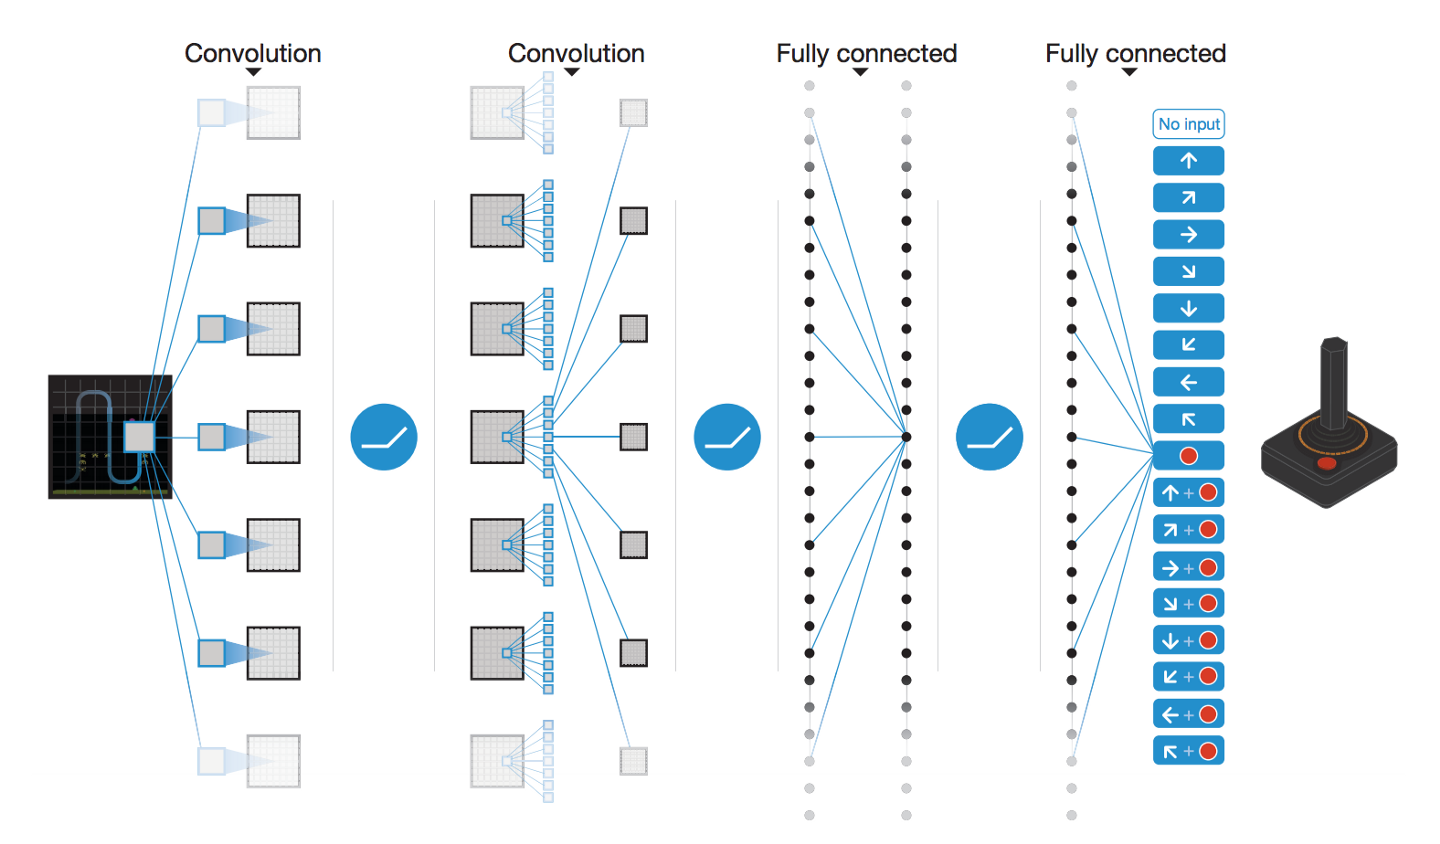
\includegraphics[scale=0.3]{network.png}
\caption{Schemat sieci neuronowej \cite{deepmind_2}}
\label{simple1}
\end{figure}

\newpage

\subsubsection{Algorytm trenowania}

\begin{lstlisting}
 initialize replay memory D
 initialize the neural network with random data
 get the current state 's'
 while game not over
 	if random > epsilon 
 		'a' = random action
 	otherwise
 		'a' = argmax_{a'}Q(s,a')

	perform action 'a'
	get reward 'r' and state 's`'
	store experience <s,a,r,s'> in memory D
	
	sample 32 random experiences <ss, aa, rr, ss'> from memory D
	for each experience from the sample batch
		if ss' is the final state 
			tt=rr
		otherwise
			tt=rr+gamma*argmax_{aa'}Q(ss', aa')
	
	optimize the neural network using loss function tt-Q(ss,aa))^2
	
	s=s'
\end{lstlisting}

\newpage

\begin{thebibliography}{9}

\bibitem{atari}
  Atari 2600 \url{https://en.wikipedia.org/wiki/Atari_2600}

\bibitem{gym}
  OpenAI Gym \url{https://gym.openai.com/}


\bibitem{deepmind_1}
  Volodymyr Mnih et al. 
\textit{Playing Atari with Deep Reinforcement Learning.} Deepmind, 2013
   \url{https://deepmind.com/research/publications/playing-atari-deep-reinforcement-learning/}

\bibitem{deepmind_2}
  Volodymyr Mnih et al. 
\textit{Human-level control through deep reinforcement learning.} Deepmind, 2015
   \url{https://deepmind.com/research/publications/human-level-control-through-deep-reinforcement-learning/}


\end{thebibliography}


\end{document}